\newpage
\section{Scale-space feature detectors}

\Cref{code:R} shows my function for computing (single-scale) Harris responses
using the formula for $R$ given in the assignment text. The function uses
\texttt{gaussian\_filter} from \texttt{scipy.ndimage} which allows for easy
convolution with (partial derivatives of) Gaussian kernels. Using this, the
function is a quite straight-forward implementation of the formulas given in
equation (2) and (3).

\begin{figure}[H]
  \centering
  \begin{minted}[fontsize=\footnotesize]{python}
from skimage.util import img_as_float
from scipy.ndimage import gaussian_filter
...
def harris_response(img, sigma, alpha = 0.05, k = 1):
    img = img_as_float(img)

    Lx  = gaussian_filter(img, sigma, order = [1, 0])
    Ly  = gaussian_filter(img, sigma, order = [0, 1])
    Axx = gaussian_filter(Lx ** 2, k * sigma)
    Axy = gaussian_filter(Lx * Ly, k * sigma)
    Ayy = gaussian_filter(Ly ** 2, k * sigma)

    det_A   = Axx * Ayy - Axy ** 2
    trace_A = Axx + Ayy
    R = sigma ** 4 * (det_A - alpha * trace_A ** 2)
    return R
  \end{minted}
  \captionof{listing}{Code for (single-scale) Harris responses using the formula for $R$ given
    in the assignment text.}
  \label{code:R}
\end{figure}

Next, \cref{code:multi_scale_corners} shows the wrapper code I use to compute
multi-scale corner detection. It is essentially just wrappers for the Harris
response function in \cref{code:R}. Note that I use \texttt{peak\_local\_max} to
compute local maxima, and that I simply use the default \texttt{min\_distance =
1}.

\begin{figure}[H]
  \centering
  \begin{minted}[fontsize=\footnotesize]{python}
def multi_scale_harris_response(img, sigmas, alpha = 0.05, k = 1):
    return np.array([harris_response(img, sigma, alpha, k)
                     for sigma in sigmas])

def multi_scale_corner_detection(img,
                                 sigmas = np.logspace(0, 5, 30, base = 2),
                                 num_peaks = 350,
                                 alpha = 0.05,
                                 k = 1):
    responses = multi_scale_harris_response(img, sigmas, alpha, k)
    peaks = peak_local_max(responses, num_peaks = num_peaks).astype(float)
    peaks[:, 0] = sigmas[peaks[:, 0].astype(int)]
    return peaks
  \end{minted}
  \captionof{listing}{Code for multi scale corner detection.}
  \label{code:multi_scale_corners}
\end{figure}


\paragraph{Running multi-scale corner detection}~\smallskip

As I understand the assignment we only need to test using a single $k$, but
multiple values for $\alpha$. Hence I choose $k = 1.5$, since I found it to be
optimal in most cases. In addition, I try various values of $\alpha$ between
0.005 and 1, including 0.05 as requested. For the range of $\sigma$-values, I
use simply the formula suggested in the assignment text (\texttt{np.logspace(0,
5, 30, base = 2)}).

\Cref{fig:task_4} shows the result of running multi-scale corner detection for
these parameters. Interestingly, the detection more or less completely fails for
$\alpha \geq 0.5$, while for the four smallest $\alpha$ values, the results are
to some degree identical: A lot of the major corners are properly detected,
while some of the smaller edges -- especially along some of the various window
panes -- are missing.


\begin{figure}[H]
  \centering
  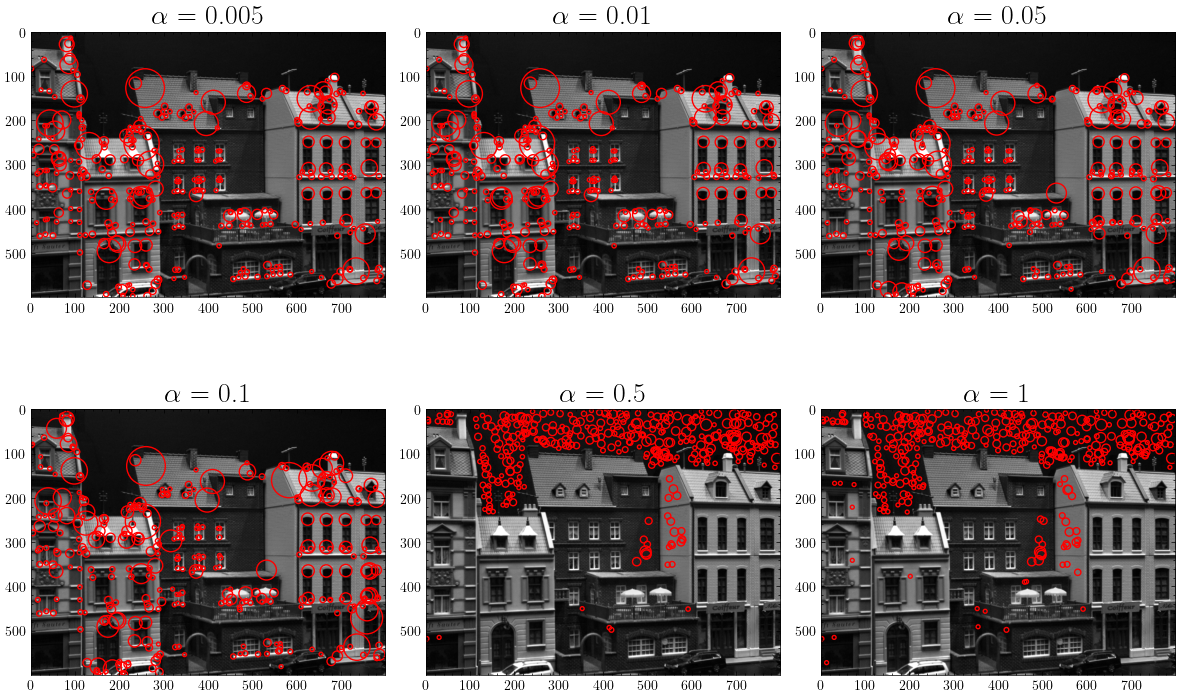
\includegraphics[width=\textwidth]{figures/task_4.png}
  \caption{Multi-scale corner detection for $k = 1.5$ and varying $\alpha$, with
  (up to) 350 local maxima for each case.}
  \label{fig:task_4}
\end{figure}
